\newpage

%\onecolumn



\section{Data Construction} %%%%%%%%%%%%%%%%%%%%%
\label{appendix:data-construction}
% % In large-scale training, redundant information increases storage and computation costs and affects the performance of RL training. 
% % To ensure the quality of the training data for RL, we screen high-quality QA data from several open-source datasets for RL training and use DeepSeek-R1 to obtain long CoT data for code start.
% % To reduce storage and computational costs while improving performance in large-scale RL training, we filter high-quality QA data from multiple open-source datasets and use DeepSeek-R1 to generate long CoT data for the cold-start.

We use part of the data extracted from NqOpen \cite{kwiatkowski2019natural,lee2019latent}, as well as data from WebQuestions \citep{berant2013semantic} and ComplexQuestions \citep{bao2016constraint}, as factual question data sources.

Initially, we filtered out trivial queries and applied semantic de-duplication to ensure data diversity. 
The remaining data underwent quality refinement and entity extraction via GPT-4o (see Appendix \ref{appendix:4o-prompt} for detailed prompts).
To address the limitation of incomplete knowledge coverage in existing datasets (e.g., HotpotQA), we explicitly matched the extracted entities against the Wikipedia dump\footnote{20231101.en, https://dumps.wikimedia.org/.} to retrieve comprehensive factual contexts for each question. 
Finally, we applied length constraints to screen the samples, resulting in a robust dataset for stable training.
% % \paragraph{Pre-processing and Simple Filtering.}
% % First of all, we filter out data with multiple possible answers because they can easily lead to unstable training. 
% % At the same time, we discard data with no obvious questioning tone, as such data can easily lead to the model not knowing the meaning of the question and thus blindly exploring it during the training process. 
% % We believe that there is no need for RL training for simple questions, so we use the Qwen2.5-7B-Instruct \citep{qwen2.5} to filter the simple data in the data source, and the filtering method is to filter out the questions that are answered correctly for the first time by the Qwen2.5-7B-Instruct.

% \paragraph{Multiple De-duplication and Entropy Filtering.}
% First, we filter questions that Qwen2.5-7B-Instruct \citep{qwen2.5} answers correctly on its first attempt. 
% The NqOpen dataset, due to its large size and less stringent prior cleaning, then undergoes de-duplication to ensure data diversity. We use Semhash on this filtered NqOpen data for both exact and semantic de-duplication, employing potion-base-8M \citep{minishlab2024model2vec} as the sentence embedding model for the semantic step. 
% Finally, this de-duplicated NqOpen data is combined with the initially filtered WebQuestions and ComplexQuestions data to form the filtered data.
% % Based on the generated semantic vectors, we use the approximate nearest neighbor search algorithm to quickly search for similar vectors, mark the data with cosine similarity greater than a threshold as similar data and form a cluster, only one sample is selected from a cluster, and the rest of the data are marked as duplicate data and filtered. 
% % According to the entropy value calculated for each problem, the top 80\% proportion of data is selected as the filtered data, thus ensuring data diversity. 


% \paragraph{Refinement and Entity Extraction.}
% In this step, we use GPT-4o and predefined rules to check the data from step 1, excluding questions that are informal, lack sufficient information for reasoning, or use informal language. 
% Guided by carefully designed prompts (see Appendix), GPT-4o accepts or rejects items and, for those accepted, normalizes, corrects, and extracts entities. 
% To ensure manageable training difficulty, DeepSeek-R1 then further filters this data, retaining only questions it answers correctly on its first attempt; this process also provides the long CoT data needed for SFT baseline training.

% % \paragraph{Difficulty Filtering.}
% % To avoid excessive difficulty in the training data, we choose to further filter the data obtained from the previous step using DeepSeek-R1, specifically selecting questions that DeepSeek-R1 answers correctly on its first attempt. 
% % This step also helped us get the long COT data needed for the SFT baseline.

% \paragraph{Wikipedia-grounded Data Filtering.}
% This step filters out data that cannot be matched to our knowledge source, Wikipedia \footnote{The English Wikipedia dump, version 20231101.en.} (6.4 million entries).
% %\footnote{20231101.en, https://dumps.wikimedia.org/.} (6.4 million entries). 
% Based on each data item's entities, we retrieve corresponding Wikipedia entries—requiring an exact entity match or full containment within a Wikipedia entry title for a successful link. We then add their textual content to our knowledge base. 
% To avoid redundancy, each entity keyword links to no more than three Wikipedia entries, and items with entities failing to match any entry are filtered out. 
% Additionally, to ensure SFT training stability, we retain only the 3,177 data items where DeepSeek-R1's output length is between 300 and 700 tokens, thus completing the training data construction.

% \subsection{Cold Start Data Construction}
% % We obtain another part of the remaining data from NqOpen and perform the same filtering steps as we did to construct the RL training data.
% % We use DeepSeek-R1 to distill the long CoT data and filter out the questions that DeepSeek-R1 answered correctly the first time. 
% % And merge the data that failed to match the knowledge in the RL training data construct as data source. 
% % Only 1798 data items with DeepSeek-R1 output length between 300 and 700 are kept as cold-start training data.
% We process another portion of NqOpen data using the same filtering method as our RL training data construction: employing DeepSeek-R1 to distill long CoT responses while retaining only first-attempt correct answers. The filtered outputs (300-700 tokens) that mismatch RL training knowledge become our cold-start dataset, yielding 1,798 qualified entries.











%\newpage


%\newpage
\section{Training Setups}
\label{appendix:train-set}

We are training two 7B models, DeepSeek-R1-Distill-Qwen-7B and Skywork-OR1-7B-Preview, with Reinforcement Learning on 1×A800. 
Detailed training hyperparameters are listed in Table~\ref{tab:training_hyperparameters}.

\begin{table}[h]
    \centering
    \small
    \setlength{\tabcolsep}{15pt} % 适当增加列间距
    \renewcommand{\arraystretch}{1.1} % 稍微增加行高
    \begin{tabular}{lc}
    \toprule
    \textbf{Parameter} & \textbf{Value} \\
    \midrule
    lora\_rank & 128 \\
    lora\_alpha & 256 \\
    torch\_dtype & bfloat16 \\
    per\_device\_train\_batch\_size & 20 \\
    gradient\_accumulation\_steps & 4 \\
    learning\_rate & 1.0e-5 \\
    beta & 0.001 \\
    lr\_scheduler\_type & cosine \\
    warmup\_ratio & 0.03 \\
    vllm\_gpu\_memory\_utilization & 0.5 \\
    optim & adamw\_8bit \\
    \bottomrule
    \end{tabular}
    \caption{Hyperparameter settings for RL training. Both DeepSeek-R1-Distill-Qwen-7B and Skywork-OR1-7B-Preview share these identical configurations.}
    \label{tab:training_hyperparameters}
\end{table}

%\newpage
% \section{ColdStart SFT Overtraining }
% To investigate the effects of prolonged ColdStart SFT, DeepSeek-R1-Distill-Qwen-7B was trained for 1200 steps in this initial stage, creating the DeepSeek-R1-Distill-Qwen-7B-ColdStart1200steps model. 
% Examination of this model's 50-step RL training curve, presented in Figure~\ref{ColdStart1200steps}, reveals a key challenge: the model exhibits significant difficulty in learning even the most basic format rewards within this RL timeframe. This observation suggests that over-training during the cold-start SFT phase can seriously diminish the efficacy of the ensuing reinforcement learning phase.

% \begin{figure*}[h]
%     \centering
%     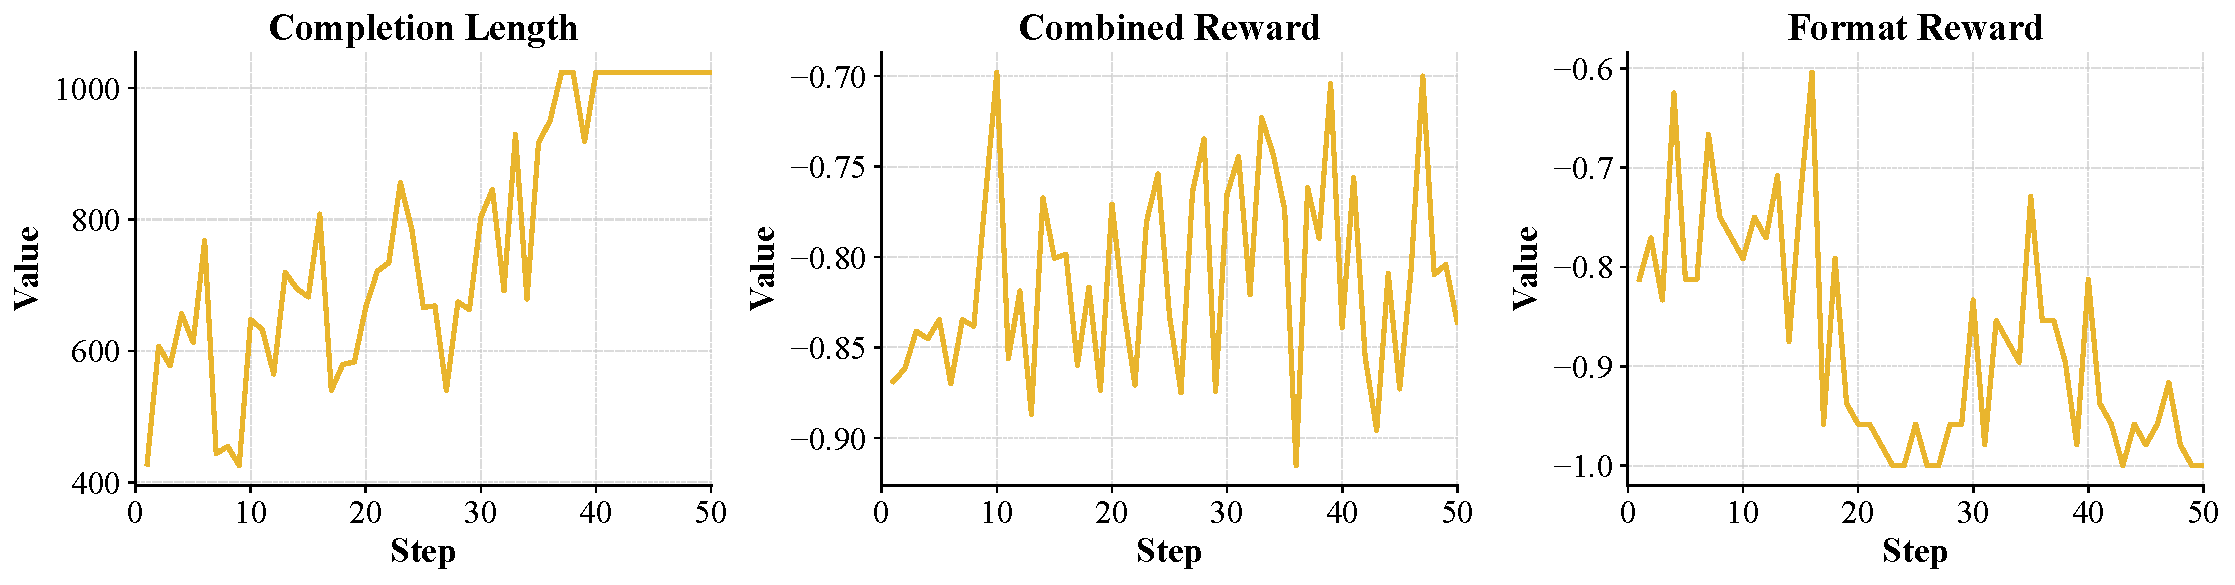
\includegraphics[width=0.95\linewidth]{images/rl-50steps.pdf}
%     \caption{DeepSeek-R1-Distill-Qwen-7B-ColdStart1200steps Training Curve.}
%     \label{ColdStart1200steps}
% \end{figure*}

% \newpage
% \section{Extended Evaluation on Reasoning Benchmarks}
% \label{appendix:extended-evaluation}
% To further demonstrate the robustness of our method on demanding reasoning tasks, we extend our evaluation beyond GPQA and AIME 2025 to include two additional challenging benchmarks: OlympiadBench and TheoremQA. These datasets test complex scientific and mathematical reasoning, requiring multi-step logical deduction far beyond simple Q\&A. The results reinforce our claim that KnowRL improves reasoning while mitigating hallucination.


% \subsection*{1. Performance on TheoremQA}
% \begin{table*}[h]
%     \small
%     %\setlength{\tabcolsep}{4pt}
%     \centering
%     \begin{tabular}{lccc}
%     \toprule
%     \textbf{Model} & \textbf{Direct Generation} & \textbf{KnowRL Trained} & \textbf{Improvement} \\
%     \midrule
%     DeepSeek-R1-Distill-Qwen-7B & 12.75\% & 17.88\% & +5.13\% \\
%     Skywork-OR1-7B-Preview    & 12.00\% & 15.12\% & +3.12\% \\
%     \bottomrule
%     \end{tabular}
%     \caption{Performance on TheoremQA.}
%     \label{tab:theoremqa}
% \end{table*}


% \subsection*{2. Performance on OlympiadBench}
% \begin{table*}[h]
%     \centering
%     \small
%     %\setlength{\tabcolsep}{4pt}
%     \begin{tabular}{lcccc}
%     \toprule
%     \textbf{Sub-task} & \textbf{DS-Base} & \textbf{DS-KnowRL} & \textbf{SW-Base} & \textbf{SW-KnowRL} \\
%     \midrule
%     maths\_en\_COMP      & 8.61\% & 9.94\% & 4.75\% & 7.42\% \\
%     maths\_zh\_COMP      & 7.35\% & 11.27\% & 5.39\% & 6.62\% \\
%     maths\_zh\_CEE       & 10.65\% & 9.35\% & 8.79\% & 8.15\% \\
%     physics\_en\_COMP    & 1.69\% & 1.27\% & 0.85\% & 0.00\% \\
%     physics\_zh\_CEE     & 7.83\% & 13.91\% & 3.48\% & 9.57\% \\
%     \bottomrule
%     \end{tabular}
%     \caption{Performance on OlympiadBench, with layout transposed for clarity. DS-Base: DeepSeek-R1-Distill-Qwen-7B, DS-KnowRL: the KnowRL-trained version. SW-Base: Skywork-OR1-7B-Preview, SW-KnowRL: the KnowRL-trained version.}
%     \label{tab:olympiadbench_transposed}
% \end{table*}

% On the TheoremQA benchmark, both the DeepSeek-R1-Distill-Qwen-7B and Skywork-OR1-7B-Preview models show significant accuracy improvements after being trained with KnowRL. On the more challenging OlympiadBench, the models trained with KnowRL exhibit only a slight performance decrease in the maths\_zh\_CEE and physics\_en\_COMP sub-tasks, while achieving considerable gains across the other tested math and physics categories. This demonstrates that KnowRL largely preserves and often enhances the models' complex reasoning capabilities.

% These new results, combined with our original findings on GPQA and AIME 2025, provide stronger evidence that our method successfully mitigates hallucination while simultaneously preserving and often enhancing the model's ability to tackle a wide array of complex, slow-thinking reasoning tasks.




%\newpage
% \section{Extended Evaluation on Diverse Model Architectures}
% \label{appendix:model-architectures}
% To test the generalizability of our framework, we extend our evaluation to two additional model types with distinct architectures: a slow-thinking model developed purely through Supervised Fine-Tuning (SFT) and a representative fast-thinking model.

% \begin{table*}[h]
% \centering
%     \small
%     %\setlength{\tabcolsep}{6pt}
%     \begin{tabular}{l|cc|cc}
%     \toprule
%     \multirow{3}{*}{\textbf{Benchmark}} & \multicolumn{2}{c|}{\textbf{OpenThinker3-7B (Slow)}} & \multicolumn{2}{c}{\textbf{Qwen2.5-7B-Instruct (Fast)}} \\
%     \cmidrule(lr){2-3} \cmidrule(lr){4-5}
%      & \textbf{Direct Generation} & \textbf{KnowRL} & \textbf{Direct Generation} & \textbf{KnowRL} \\
%     \midrule
%     TruthfulQA          & 38.19\% & 36.60\% & 30.97\% & 40.51\% \\
%     SimpleQA            & 3.55\%  & 7.61\%  & 4.09\%  & 3.29\%  \\
%     ChineseSimpleQA     & 15.67\% & 18.97\% & 29.00\% & 27.70\% \\
%     GPQA Diamond        & 28.28\% & 37.88\% & 35.86\% & 37.88\% \\
%     AIME2025            & 10.00\% & 20.00\% & 6.67\%  & 10.00\% \\
%     \bottomrule
%     \end{tabular}
%     \caption{Comparative performance of KnowRL on an SFT-based slow-thinking model (OpenThinker3-7B) and a fast-thinking model (Qwen2.5-7B-Instruct).}
%     \label{tab:Diverse_Model}
% \end{table*}

% As shown in Table~\ref{tab:Diverse_Model}, for the SFT-based slow-thinking model, OpenThinker3-7B, applying KnowRL yields substantial gains across both reasoning and factuality benchmarks. Performance on reasoning tasks like GPQA Diamond surges from 28.28\% to 37.88\%, and the score on AIME2025 doubles. Simultaneously, its factuality on datasets like SimpleQA and ChineseSimpleQA improves significantly.

% In contrast, the results on the fast-thinking model, Qwen2.5-7B-Instruct, are more nuanced. While the model's complex reasoning (AIME 2025) and truthfulness on a challenging dataset (TruthfulQA) improve after KnowRL training, its performance on simpler factual recall datasets (SimpleQA, ChineseSimpleQA) declines. This suggests a trade-off where imposing a deliberate, step-by-step reasoning process on a model optimized for rapid responses enhances complex logic at the cost of simple recall efficiency.

% In comparing these outcomes, it becomes clear that KnowRL's mechanism—rewarding a verifiable, step-by-step thinking process—aligns more naturally with the architecture of slow-thinking models, which is highly consistent with our paper's original motivation to solve the hallucination problem inherent to these models. Therefore, this comparative analysis leads us to a more refined conclusion: KnowRL is not as well-suited for trying to build up a model's reasoning skills and its ability to follow facts at the same time, from scratch. Rather, it is well-suited for models that are already good at 'slow thinking', as its primary role is to teach them how to reason based on facts while preserving their existing reasoning abilities.



\section{Case Analysis}
To explore KnowRL's impact on reasoning in factual tasks, we analyzed a reasoning case from the KnowRL training process, detailing the model's emergent reasoning behaviors. As shown in Figure~\ref{case}, these include Mixed-Language Reasoning, Knowledge Anchoring, Cross-verification, and Key Information Extraction. For simple factual tasks, distinct from mathematical reasoning, the model typically first proposes an initial answer (knowledge anchoring) and subsequently verifies this initial answer through reasoning behaviors such as reflection and cross-verification. This observed process aligns with human cognitive approaches when facing factual tasks, which further suggests the suitability of an outcome-based, reward-driven reinforcement learning training paradigm for open-domain factual tasks.

\begin{figure}[t]
    \centering
    \resizebox{0.48\textwidth}{!}{
    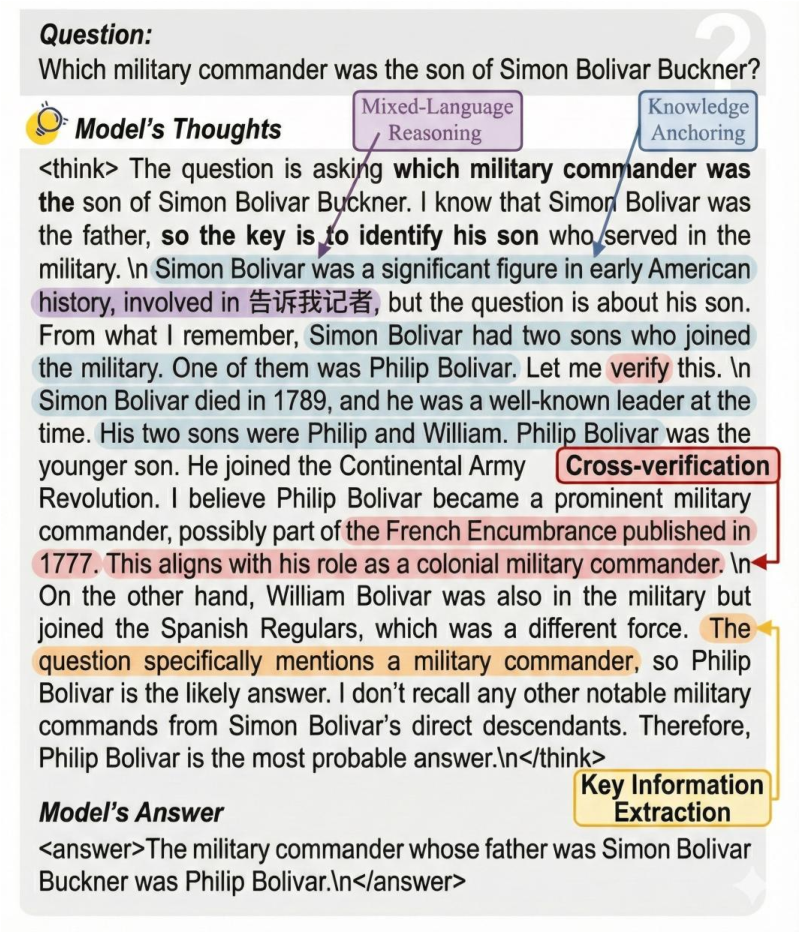
\includegraphics{images/new_case.pdf}}
    \caption{Case analysis of the KnowRL training process.}
    \vspace{-3ex}
     \label{case}
\end{figure}


\section{Training Dynamics of Different RL Algorithms}

\label{appendix:RL_algorithms}
As shown in Figure~\ref{fig:reward_comparison}, the reward curves for all four algorithms rise and stabilize, indicating successful convergence. 
Figure~\ref{fig:RL_algorithms} illustrates the training dynamics of the DeepSeek-R1-Distill-Qwen-7B model using BNPO, DAPO, and Dr.GRPO. A key observation is that all three algorithms effectively help the model establish clear knowledge boundaries to avoid hallucination. This effectiveness is evidenced by the rapid decline in completion length across all methods. The sharp drop indicates a behavioral shift where the model learns to provide concise refusals instead of generating long and potentially fabricated responses. This consistent pattern confirms that these RL approaches successfully guide the model toward reliable behavior and mitigate uncontrolled generation. Despite these shared trends, the algorithms differ in training efficiency and their impact on factual reasoning.



\begin{figure*}[t]
    \centering
    % --- 第一张图：BNPO ---
    \begin{subfigure}[b]{0.32\textwidth}
        \centering
        % 建议检查文件名：这里是 BNPO，但你之前的 caption 写的是 Skywork，请确认图片内容
        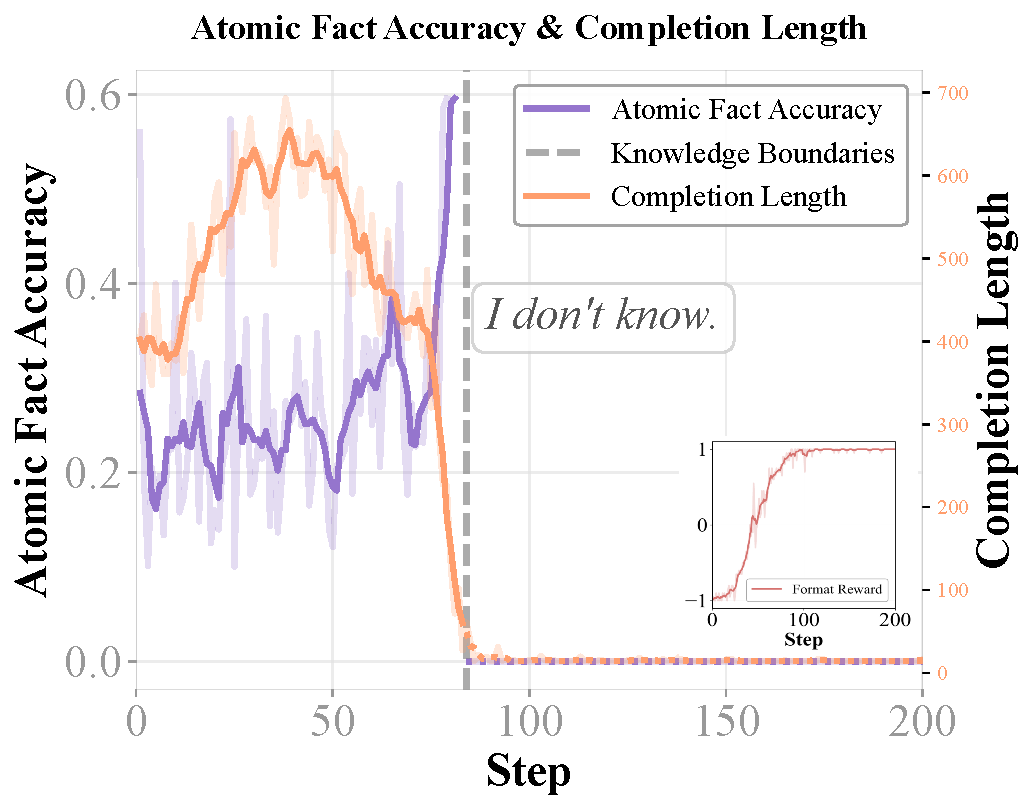
\includegraphics[width=\linewidth]{images/DeepSeek_BNPO.pdf}
        \caption{\textbf{BNPO}} 
        \label{fig:train_bnpo}
    \end{subfigure}
    \hfill % 弹性间距，让三张图撑满一行
    % --- 第二张图：DAPO ---
    \begin{subfigure}[b]{0.32\textwidth}
        \centering
        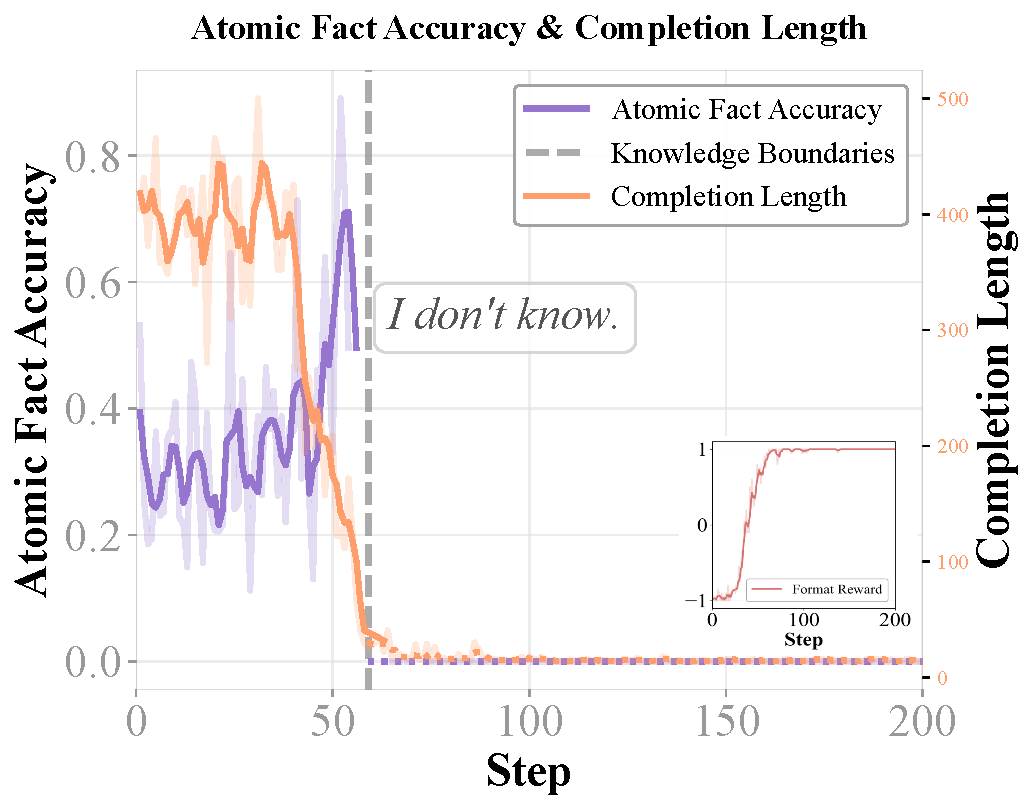
\includegraphics[width=\linewidth]{images/DeepSeek_DAPO.pdf}
        \caption{\textbf{DAPO}}
        \label{fig:train_dapo}
    \end{subfigure}
    \hfill
    % --- 第三张图：Dr.GRPO ---
    \begin{subfigure}[b]{0.32\textwidth}
        \centering
        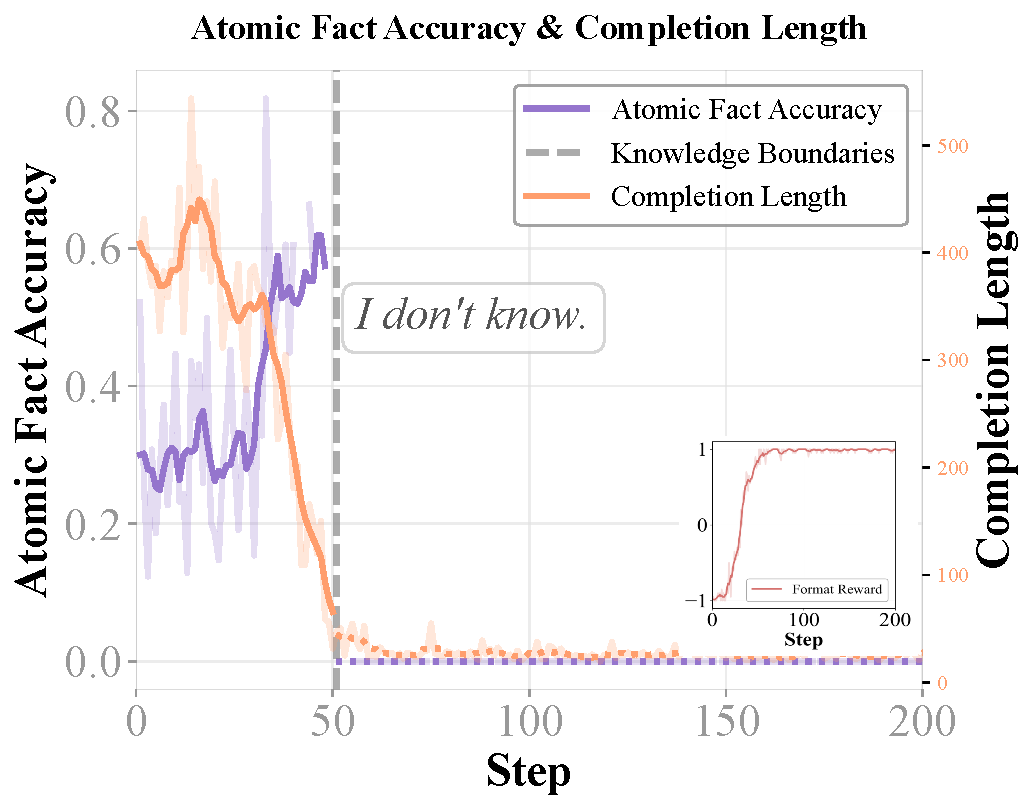
\includegraphics[width=\linewidth]{images/DeepSeek_DR.GRPO.pdf}
        \caption{\textbf{Dr.GRPO}}
        \label{fig:train_drgrpo}
    \end{subfigure}

    % --- 主标题：统一解释 ---
    \caption{
        \textbf{Training Dynamics on DeepSeek-R1-Distill-Qwen-7B.} 
        We visualize the training curves of different RL algorithms: (a) BNPO, (b) DAPO, and (c) Dr.GRPO. 
    }
    \vspace{-3ex} % 减少图片与正文的距离，节省版面
    \label{fig:RL_algorithms}
\end{figure*}




\section{Scalability Analysis on Larger Models}
\label{appendix:scalability}

We further evaluate the scalability of KnowRL by extending our experiments to the DeepSeek-R1-Distill-Qwen-14B model. As illustrated in Table~\ref{tab:perf_transposed}, KnowRL maintains its efficacy in mitigating hallucinations while simultaneously enhancing reasoning capabilities. Notably, on SimpleQA, our method significantly reduces the Incorrect Rate from 83.00\% to 68.33\% while doubling the Refusal Rate (13.33\% to 26.33\%). This shift indicates that the model acquires a more precise awareness of knowledge boundaries on larger architectures. Furthermore, KnowRL preserves and even strengthens complex reasoning performance, evidenced by the improvement in GPQA Diamond accuracy from 46.97\% to 51.01\%. These results validate that the benefits of our approach are robust and scalable across different model sizes.

\begin{figure}[h]
    \centering
    \resizebox{.425\textwidth}{!}{
    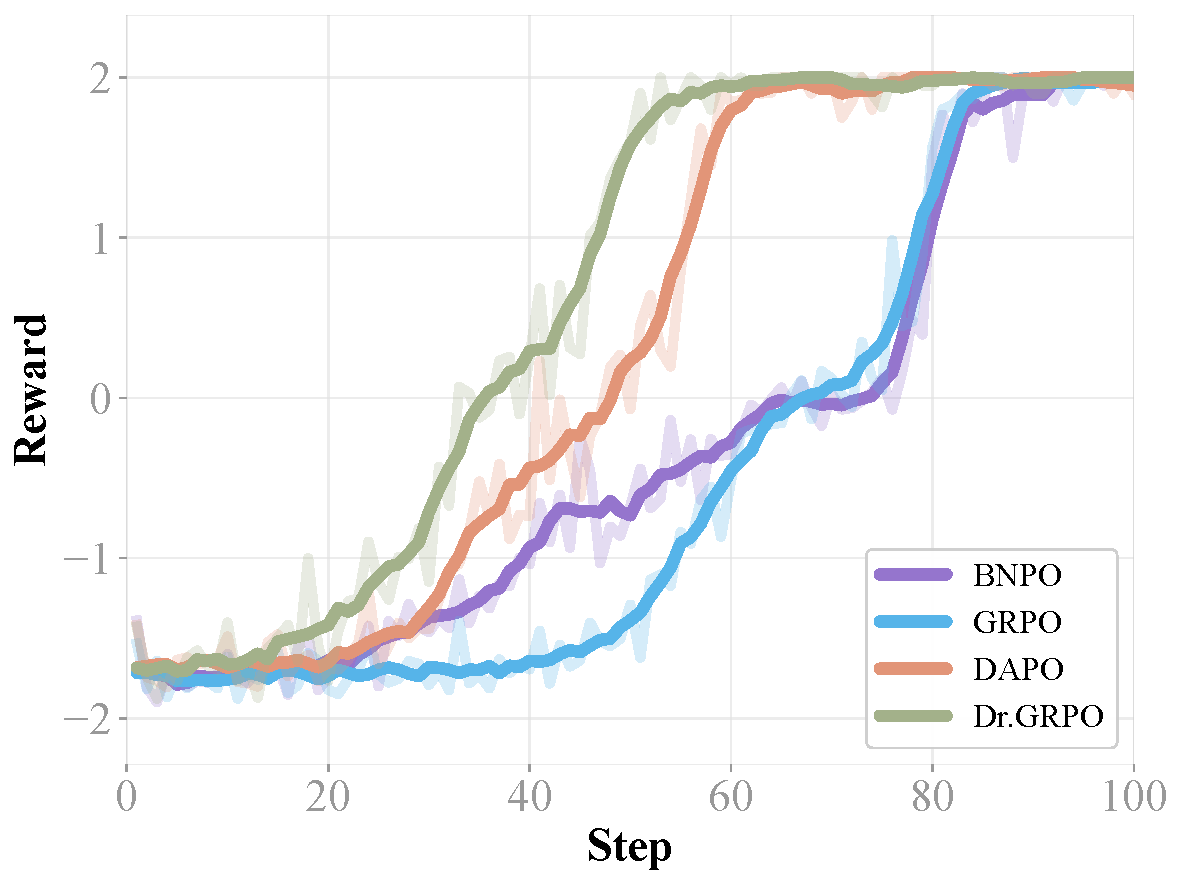
\includegraphics{images/combined_reward_comparison.pdf}}
    \caption{
    Comparison of training reward curves across different algorithms.}
    \vspace{-3ex}
    \label{fig:reward_comparison}
\end{figure}

\begin{table}[h]
    \centering
    \small
    \setlength{\tabcolsep}{13pt} % 稍微增加列间距，提升阅读舒适度
    \renewcommand{\arraystretch}{0.9} % 增加行高，避免拥挤
    \begin{tabular}{lcc}
    \toprule
    \textbf{Metric} & \textbf{Zero-shot} & \textbf{KnowRL} \\
    \midrule
    \multicolumn{3}{l}{\textit{TruthfulQA}} \\
    \quad Rouge & 53.33 & 54.67 \\
    \quad Bleu  & 50.33 & 55.00 \\
    \addlinespace[2pt] % 增加一点组间距
    \multicolumn{3}{l}{\textit{SimpleQA}} \\
    \quad PAQ & 4.23 & 6.17 \\
    \quad Incorrect & 83.00 & 68.33 \\
    \quad Refusal & 13.33 & 26.33 \\
    \quad F1 & 3.93 & 6.14 \\
    \addlinespace[3pt]
    \multicolumn{3}{l}{\textit{ChineseSimpleQA}} \\
    \quad PAQ & 29.18 & 31.07 \\
    \quad Incorrect & 63.33 & 61.33 \\
    \quad Refusal & 6.33 & 11.00 \\
    \quad F1 & 28.23 & 29.28 \\
    \addlinespace[3pt]
    \multicolumn{3}{l}{\textit{GPQA Diamond}} \\
    \quad Accuracy & 46.97 & 51.01 \\
    \addlinespace[3pt]
    \multicolumn{3}{l}{\textit{AIME}} \\
    \quad Accuracy & 40.00 & 36.67 \\
    \bottomrule
    \end{tabular}
    \caption{Performance comparison on DeepSeek-R1-Distill-Qwen-14B. The results demonstrate that KnowRL consistently improves hallucination mitigation (SimpleQA) and reasoning (GPQA) compared to the Zero-shot baseline.}
    \label{tab:perf_transposed}
\end{table}





\section{Evaluator Sensitivity Analysis}
\label{appendix:sensitivity}



\begin{table}[H]
    \centering
    \small
    \setlength{\tabcolsep}{5.5pt} % 增加列间距
    \renewcommand{\arraystretch}{0.9} % 增加行高
    \begin{tabular}{lcc}
    \toprule
    \textbf{Metric} & \textbf{Qwen2.5-72B-Instruct} & \textbf{GPT-4o-mini} \\
    \midrule
    \multicolumn{3}{l}{\textit{TruthfulQA}} \\
    \quad Rouge & 57.00 & 57.33 \\
    \quad Bleu  & 53.67 & 51.60 \\
    \addlinespace[2pt]
    \multicolumn{3}{l}{\textit{SimpleQA}} \\
    \quad PAQ & 1.53 & 2.81 \\
    \quad Incorrect & 64.33 & 57.67 \\
    \quad Refusal & 34.67 & 40.67 \\
    \quad F1 & 1.21 & 2.09 \\
    \addlinespace[3pt]
    \multicolumn{3}{l}{\textit{ChineseSimpleQA}} \\
    \quad PAQ & 9.74 & 10.26 \\
    \quad Incorrect & 58.67 & 58.33 \\
    \quad Refusal & 35.00 & 35.00 \\
    \quad F1 & 7.68 & 8.08 \\
    \addlinespace[3pt]
    \multicolumn{3}{l}{\textit{GPQA Diamond}} \\
    \quad Accuracy & 38.38 & 36.87 \\
    \addlinespace[3pt]
    \multicolumn{3}{l}{\textit{AIME}} \\
    \quad Accuracy & 33.33 & 33.33 \\
    \bottomrule
    \end{tabular}
    \caption{Robustness analysis of KnowRL using different evaluator models during training.}
    \label{tab:evaluator_comparison}
\end{table}

To confirm that the effectiveness of KnowRL is not dependent on a specific reward model used during training (e.g., GPT-4o-mini), we conducted an ablation study by replacing it with Qwen2.5-72B-Instruct \citep{qwen2.5}. 
As presented in Table~\ref{tab:evaluator_comparison}, the results demonstrate that KnowRL maintains comparable performance across different evaluators. 
Specifically, we observe that the model trained with GPT-4o-mini exhibits more conservative behavior, achieving a higher Refusal Rate and a lower Incorrect Rate on SimpleQA. In contrast, using Qwen2.5-72B-Instruct yields slightly higher performance on reasoning-heavy benchmarks like GPQA Diamond, suggesting a subtle trade-off between strict factuality enforcement and reasoning preservation depending on the evaluator's characteristics. 
This confirms that the efficacy of our method stems from the intrinsic KnowRL framework rather than reliance on a specific external judge.





\section{Evaluation of Generative Diversity}
\label{app:generative_diversity}

To investigate whether KnowRL's boundary-aware training inadvertently leads to over-conservatism or a loss of generative diversity, we evaluate our models using NoveltyBench \cite{zhang2025noveltybench}. This benchmark measures the ability of LLMs to produce diverse outputs for the same prompt. We conduct evaluations on the \textit{nb-curated} (100 prompts) and \textit{nb-wildchat} (1,000 prompts) subsets, sampling 10 responses per prompt at a temperature of 0.6. We report the \textit{distinct} metric, which averages the number of semantically unique equivalence classes across generations.

\begin{table}[h]
    \centering
    \small
    \setlength{\tabcolsep}{5.5pt} 
    \renewcommand{\arraystretch}{0.9} 
    \begin{tabular}{lcc}
    \toprule
    \textbf{Model} & \textbf{nb-curated} & \textbf{nb-wildchat} \\
    \midrule
    DeepSeek-7B & 1.61 & 1.71 \\
    DeepSeek-7B + KnowRL & 1.54 & 1.74 \\
    \midrule
    Skywork-7B & 1.63 & 1.65 \\
    Skywork-7B + KnowRL & 1.68 & 1.64 \\
    \bottomrule
    \end{tabular}
    \caption{Generative diversity (\textit{distinct} scores) on NoveltyBench subsets.}
    \label{tab:noveltybench}
\end{table}

As shown in Table \ref{tab:noveltybench}, the variation in \textit{distinct} scores after KnowRL training is extremely marginal ($\pm 0.01$ to $\pm 0.07$), indicating that the model's generative diversity remains intact. We attribute this preservation to the use of Low-Rank Adaptation (LoRA), which allows the model to learn new boundary-aware behaviors while mitigating the catastrophic forgetting of its original generative capabilities. While KnowRL increases refusal rates for out-of-knowledge queries to reduce hallucinations, it does not compromise the model's creative breadth in open-ended scenarios. We note that establishing an absolute ``False Refusal Rate'' remains challenging due to the difficulty of probing a model's precise internal knowledge, which we leave for future investigation.






\section{Implementation Details for Baselines}
\label{app:baseline_details}

To ensure fair comparison and reproducibility, all trainable baselines are fine-tuned using Low-Rank Adaptation (LoRA) and utilize the exact same QA training dataset as KnowRL.
The specific implementation details for each baseline are described as follows:

\begin{itemize}
    \item \textbf{Self-Refine (Prompt Engineering):} The model generates an initial response and then performs self-critique to provide feedback.
    It uses this self-feedback to refine its output iteratively.
    This ``FEEDBACK $\rightarrow$ REFINE'' loop is repeated until a stopping condition is met, specifically when it reaches a maximum of 5 iterations or when the model determines that no further improvement is needed.
    
    \item \textbf{SFT (Supervised Fine-Tuning):} We train the model using the correct reasoning processes and final answers distilled from the DeepSeek-R1 model as the target outputs.
    
    \item \textbf{DPO (Direct Preference Optimization):} We construct the preference pairs by using the correct answer distilled from DeepSeek-R1 as the ``chosen'' response, and the model's own incorrect generation as the ``rejected'' response.
    
    \item \textbf{FactTune-FS:} Following the methodology of the original paper \cite{REPLACE_WITH_FACTTUNE_CITATION}, we sample multiple responses from the model for a given prompt and evaluate them using FactScorer.
    We then construct DPO training pairs by selecting two responses that have a FactScore difference greater than 0.8.
    
    \item \textbf{TruthRL:} We adopt the exact same GRPO training setup as KnowRL to ensure a strictly fair comparison.
    We only change the reward function to match TruthRL's original design: $+1$ for a correct answer, $0$ for a refusal, and $-1$ for an incorrect answer.
\end{itemize}












%\onecolumn


\section{Prompts}

\label{appendix:4o-prompt}



\begin{tcolorbox}[breakable,title=Prompt Used by the GPT-4o for Data Filtering]

\columnseprule=0.5pt

You are an entity extraction assistant that identifies key entities in questions.





TASK:



1. First normalize the query by properly capitalizing names, titles, and other named entities



2. Determine if the query has sufficient context to be answered meaningfully



3. Extract only the most important entities from the query that are essential for answering it





RULES:



1. Extract a MAXIMUM of 2 specific entities (people, places, objects, works, etc.)



2. Output the MOST important entity first, then the secondary entity (if any)



3. Extract precise named entities, not general concepts or phrases



4. Keep related entities together as a single entity (e.g., character names with their roles)



5. Return individual entities rather than relationships or possessive forms



6. Only extract truly representative entities - ignore generic terms that don't specifically define the query



7. Only REJECT queries that meet the rejection criteria below



ONLY reject queries in these specific cases:



1. When the entity in the query is completely ambiguous (e.g., "Who is that person?")



2. When the query lacks necessary qualifying information (e.g., "Who will win?" with no mention of what contest)



3. When the query is too vague to determine its intent (e.g., "What happened to him?")



4. When the query is time-sensitive and contains temporal references like "now", "current", "latest", "recent", etc.



5. When the query lacks sufficient information to determine a single definitive answer, potentially leading to multiple correct interpretations or answers



6. Be careful not to extract purely numerical information such as a year as an entity





Note: Queries with historical context, pop culture references, geographical locations, or other well-defined entities should be ACCEPTED.





EXAMPLES:





Example 1:



Original Query: "who played barbara gordon batgirl?"



Normalized Query: "Who played Barbara Gordon Batgirl?"



Output: Normalized Query: "Who played Barbara Gordon Batgirl?"



      Entities: ["Barbara Gordon Batgirl"]

      

NOT: ["Barbara Gordon", "Batgirl"] - This is incorrect because "Barbara Gordon 

Batgirl" is a single character entity.



Example 2:



Original Query: "what continent does armenia belong to?"



Normalized Query: "What continent does Armenia belong to?"



Output: Normalized Query: "What continent does Armenia belong to?"



      Entities: ["Armenia"]

      

NOT: ["Armenia", "continent"] - The term "continent" is a generic category, not a specific entity representative of this query.





Example 3:



Original Query: "who is niall ferguson's wife?"



Normalized Query: "Who is Niall Ferguson's wife?"



Output: Normalized Query: "Who is Niall Ferguson's wife?"



      Entities: ["Niall Ferguson"]

      



Example 4:



Original Query: "who was the italian leader in ww1?"



Normalized Query: "Who was the Italian leader in WW1?"



Output: Normalized Query: "Who was the Italian leader in WW1?"



      Entities: ["Italian leader", "WW1"]



Example 5:



Original Query: "who will play mr gray in the film?"



Normalized Query: "Who will play Mr. Gray in the film?"



Output: Normalized Query: "Who will play Mr. Gray in the film?"



      REJECT (insufficient context - which film?)





Example 6:



Original Query: "who is in charge of libya now?"



Normalized Query: "Who is in charge of Libya now?"



Output: Normalized Query: "Who is in charge of Libya now?"



      REJECT (time-sensitive query with temporal reference "now")

      



Example 7:



Original Query: "what did werner heisenberg discover?"



Normalized Query: "What did Werner Heisenberg discover?"



Output: Normalized Query: "What did Werner Heisenberg discover?"



      REJECT (lacks sufficient specificity - Heisenberg made multiple discoveries)



Please try to output in this format:



Normalized Query: "The normalized version of the query"



Entities: ["entity1", "entity2"]



If you need to reject, still include the normalized query:



Normalized Query: "The normalized version of the query"



REJECT (reason for rejection)



Extract key entities from this query: "{query}"



\end{tcolorbox}















